% Author: Alfredo Sánchez Alberca (asalber@ceu.es)
\section{Analytic geometry}

%---------------------------------------------------------------------slide----
\begin{frame}
\frametitle{Analytic geometry}
\setlength{\parskip}{0.3em}
\tableofcontents[sectionstyle=show/hide,hideothersubsections]
\end{frame}

\subsection{Vectors}

%---------------------------------------------------------------------slide----
\begin{frame}
\frametitle{Scalars}
Some phenomena of Nature can be described by a number and a unit of measurement. 

\begin{definition}[Scalar]
A \emph{scalar} is a number that expresses a magnitude without direction.
\end{definition}
\structure{\bfseries Examples} The height or weight of a person, the temperature of a gas or the time it takes a vehicle to travel a distance.

However, there are other phenomena that cannot be described adequately by a scalar. 
If, for instance, a sailor wants to head for seaport and only knows the intensity of wind, he won't know what direction to take. The description of wind requires two elements: intensity and direction. 
\end{frame}


%---------------------------------------------------------------------slide----
\begin{frame}
\frametitle{Vectors}
\begin{definition}[Vector]
A \emph{vector} is a number that expresses a magnitude and has associated an orientation and a sense.
\end{definition}

\structure{\bfseries Examples} The velocity of a vehicle or the force applied to an object. 

Geometrically, a vector is represented by an directed line segment, that is, an arrow. 
\begin{center}
\tikzsetnextfilename{analytic_geometry/vector}
% Author: Alfredo Sánchez Alberca (asalber@ceu.es)
\begin{tikzpicture}
\draw [vector] (0,0) node[anchor=south east]  {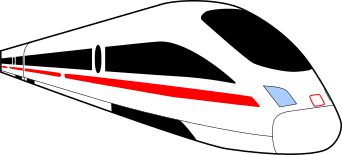
\includegraphics[scale=0.4]{img/analytic_geometry/train}} -- (2,-0.5) node[black, above, midway] {$\vec{v}$} node[sloped, pos=1, anchor=west] {direction};
\draw [decorate, decoration={brace, amplitude=5pt, mirror}, xshift=-2pt, yshift=-2pt] (0,0) -- (2,-0.5) node [midway, below, sloped, xshift=-2pt, yshift=-2pt] {magnitude};
\end{tikzpicture}

\end{center}
\end{frame}


% ---------------------------------------------------------------------slide----
\begin{frame}
\frametitle{Vector representation}
An oriented segment can be located in different places in a Cartesian space.  
However, regardless of where it is located, if the length and the direction of the segment does not change, the segment represents always the same vector. 

This allows to represent all vectors with the same origin, the origin of the Cartesian coordinate system.
Thus, a vector can be represented by the Cartesian \emph{coordinates} of its final end in any Euclidean space.

\begin{center}
\tikzsetnextfilename{analytic_geometry/vector_coordinates}
% Author: Alfredo Sánchez Alberca (asalber@ceu.es)
\begin{tikzpicture}[trim axis left, trim axis right]
  \begin{axis}[
    gen2dfun, 
    xmin=-4, xmax=4,
    ymin=-4, ymax=4,  
    xtick={3},
    xticklabels={$x_0$},
    ytick={2},
    yticklabels={$y_0$}, 
    clip=false,
    height=4cm,
    ]
    \coordinate (O) at (0,0);
    \coordinate (A) at (3,2);
    \draw[vector] (O) -- (A) node[midway, below, anchor=west] {$\mathbf{v}=(x_0,y_0)=\vec{AB}=\vec{CD}=\vec{EF}$} ;
    \draw[gray, dotted] (A) -- (A|-O);
    \draw[gray, dotted] (A) -- (A-|O);
    \draw[->] (2,2) -- (5,4) node[midway, above] {$\vec{AB}$};
    \draw[->] (-4,1) -- (-1,3) node[midway, above] {$\vec{CD}$};
    \draw[->] (-2,-3) -- (1,-1) node[midway, above] {$\vec{EF}$};
  \end{axis}
\end{tikzpicture}

\end{center}
\end{frame}


% ---------------------------------------------------------------------slide----
\begin{frame}
\frametitle{Vector from two points}
Given two points $P$ and $Q$ of a Cartesian space, the vector that starts at $P$ and ends at $Q$ has coordinates 
$\vec{PQ}=Q-P$.

\structure{\bfseries Example} Given the points $P=(1,1)$ and $Q=(3,4)$ in the real plane $\mathbb{R}^2$, the coordinates of the vector that start at $P$ and ends at $Q$ are
\[
\vec{PQ} = Q-P = (3,4)-(1,1) = (3-2,4-1) = (2,3).
\]
\begin{center}
\tikzsetnextfilename{analytic_geometry/vector_from_two_points}
% Author: Alfredo Sánchez Alberca (asalber@ceu.es)
\begin{tikzpicture}[trim axis left, trim axis right]
  \begin{axis}[
    2dfun, 
    xmin=-4, xmax=4,
    ymin=-4, ymax=4,  
    equal axis=true,
    height=4cm,
    ]
    \coordinate (0) at (0,0);
    \coordinate (P) at (2,1);
    \coordinate (Q) at (3,4);
    \draw[->, color1] (O) -- (A) node[midway, below, anchor=west] {$\vec{PQ}=(1,3)$} ;
    \draw[gray, dotted] (P) -- (P|-O);
    \draw[gray, dotted] (P) -- (P-|O);
    \draw[gray, dotted] (Q) -- (Q|-O);
    \draw[gray, dotted] (Q) -- (Q-|O);
  \end{axis}
\end{tikzpicture}

\end{center}
\end{frame}


% ---------------------------------------------------------------------slide----
\begin{frame}
\frametitle{Module of a vector}
\begin{definition}[Module of a vector]
Given a vector $\mathbf{v}=(v_1,\cdots,v_n)$ in $\mathbb{R}^n$, the \emph{module} of $\mathbf{v}$ is
\[
|\mathbf{v}| = \sqrt{v_1^2+ \cdots + v_n^2}.
\]
\end{definition}
The module of a vector coincides with the length of the segment that represents the vector.

\structure{\bfseries Examples}
Let $\mathbf{u}=(3,4)$ be a vector in $\mathbb{R}^2$, then its module is
\[
|\mathbf{u}| = \sqrt{3^2+4^2} = \sqrt{25} = 5
\]
Let $\mathbf{v}=(4,7,4)$ be a vector in $\mathbb{R}^3$, then its module is
\[
|\mathbf{v}| = \sqrt{4^2+7^2+4^2} = \sqrt{81} = 9
\]
\end{frame}


% ---------------------------------------------------------------------slide----
\begin{frame}
\frametitle{Unit vectors}
\begin{definition}[Unit vector]
A vector $\mathbf{v}$ in $\mathbb{R}^n$ is a \emph{unit vector} if its module is one, that is, $|\mathbf{v}|=1$.
\end{definition}

The unit vectors with the direction of the coordinate axes are of special importance and they form the \emph{standard basis}.

\begin{columns}
\begin{column}{.48\textwidth}
In $\mathbb{R}^2$ the standard basis is formed by two vectors
\[
\mathbf{i}=(1,0)\mbox{ and }\mathbf{j}=(0,1)
\]
\begin{center}
\tikzsetnextfilename{analytic_geometry/standard_basis_plane}
% Author: Alfredo Sánchez Alberca (asalber@ceu.es)
\begin{tikzpicture}[trim axis left, trim axis right]
  \begin{axis}[
    2dfun, 
    xmin=-0.2, xmax=2,
    ymin=-0.20, ymax=2, 
    axis equal=true,
    clip=false,
    height=3cm,
    ]
    \draw[vector] (0,0) -- (1,0) node[midway, above] {$\mathbf{i}$};
    \draw[vector] (0,0) -- (0,1) node[midway, right] {$\mathbf{j}$};
  \end{axis}
\end{tikzpicture}

\end{center}
\end{column}
\begin{column}{.48\textwidth}
In $\mathbb{R}^3$ the standard basis is formed by three vectors
\[
\mathbf{i}=(1,0,0)\mbox{, }\mathbf{j}=(0,1,0) \mbox{ and } \mathbf{k}=(0,0,1)
\]
\begin{center}
\tikzsetnextfilename{analytic_geometry/standard_basis_space}
% Author: Alfredo Sánchez Alberca (asalber@ceu.es)
\begin{tikzpicture}
  \begin{axis}[
  3dfun,
  xmin=-0.2, xmax=2,
  ymin=-0.2, ymax=2,
  zmin=-0.2, zmax=2,
  axis x line=middle,
  axis y line=middle,
  axis z line=middle,
  %axis equal=true,
  every axis x label/.style={at={(ticklabel cs:1)}, anchor=center,},
  every axis y label/.style={at={(ticklabel cs:1)}, anchor=center,},
  every axis z label/.style={at={(ticklabel cs:1)}, anchor=center,},
  clip=false,
  height=4cm,
  ]
  %\addplot3+[domain=0:pi, samples y=0] ({cos(deg(x))}, {sin(deg(x))}, {x});
  \coordinate (P) at (0,1,0);
  \draw [vector] (0,0,0) -- (1,0,0) node[anchor=west] {$\textbf{i}$};
  \draw [vector] (0,0,0) -- (0,1,0) node[anchor=west] {$\textbf{j}$};
  \draw [vector] (0,0,0) -- (0,0,1) node[anchor=west] {$\textbf{k}$};
  \end{axis}
\end{tikzpicture}

\end{center}
\end{column}
\end{columns}
\end{frame}


% ---------------------------------------------------------------------slide----
\begin{frame}
\frametitle{Sum of two vectors}
\begin{definition}[Sum of two vectors]
Given two vectors $\mathbf{u}=(u_1,\cdots,u_n)$ y $\mathbf{v}=(v_1,\cdots,v_n)$ de $\mathbb{R}^n$, the \emph{sum} of $\mathbf{u}$ and $\mathbf{v}$ is
\[
\mathbf{u}+\mathbf{v} = (u_1+v_1,\ldots, u_n+v_n).
\]
\end{definition}

\structure{\bfseries Example}
Let $\mathbf{u}=(3,1)$ and $\mathbf{v}=(2,3)$ two vectors in $\mathbb{R}^2$, then the sum of them is 
\[
\mathbf{u}+\mathbf{v} = (3+2,1+3) = (5,4).
\]

\begin{center}
\tikzsetnextfilename{analytic_geometry/sum_vectors}
% Author: Alfredo Sánchez Alberca (asalber@ceu.es)
\begin{tikzpicture}[trim axis left, trim axis right]
  \begin{axis}[
    gen2dfun, 
    xmin=0, xmax=4.5,
    ymin=0, ymax=4,
    xtick={1,3,4},
    xticklabels={$v_1$,$u_1$,$u_1+v_1$},
    ytick={1,2,3},
    yticklabels={$u_2$,$v_2$,$u_2+v_2$}, 
    %axis equal=true,
    clip=false,
    height=3cm,
    ]
    \coordinate (O) at (0,0);
    \coordinate (A) at (3,1);
    \coordinate (B) at (1,2);
    \coordinate (C) at ($(A)+(B)$);
    \draw[vector] (O) -- (A) node[midway, below] {$\mathbf{u}$} ;
    \draw[vector] (O) -- (B) node[midway, above] {$\mathbf{v}$} ;
    \draw[vector, color2] (O) -- (C) node[midway, above, sloped] {$\mathbf{u}+\mathbf{v}$} ;
    \draw[gray, dotted] (A) -- (A|-O);
    \draw[gray, dotted] (A) -- (A-|O);
    \draw[gray, dotted] (B) -- (B|-O);
    \draw[gray, dotted] (B) -- (B-|O);
    \draw[gray, dotted] (C) -- (C|-O);
    \draw[gray, dotted] (C) -- (C-|O);
    \draw[gray, dashed] (A) -- (C);
    \draw[gray, dashed] (B) -- (C);
  \end{axis}
\end{tikzpicture}

\end{center}
\end{frame}


%---------------------------------------------------------------------slide----
\begin{frame}
\frametitle{Product of a vector by an scalar}
\begin{definition}[Product of a vector by an scalar]
Given a vector $\mathbf{v}=(v_1,\cdots,v_n)$ in $\mathbb{R}^n$, and a scalar $a\in \mathbb{R}$, the \emph{product} of $\mathbf{v}$ by $a$ is 
\[
a\mathbf{v} = (av_1,\ldots, av_n).
\]
\end{definition}
\structure{\bfseries Example}
Let $\mathbf{v}=(2,1)$ a vector in $\mathbb{R}^2$ and $a=2$ a scalar, then the product of $a$ by $\mathbf{v}$ is
\[
a\mathbf{v} = 2(2,1) = (4,2).
\]

\begin{center}
\tikzsetnextfilename{analytic_geometry/product_vector_by_scalar}
% Author: Alfredo Sánchez Alberca (asalber@ceu.es)
\begin{tikzpicture}[trim axis left, trim axis right]
  \begin{axis}[
    gen2dfun, 
    xmin=0, xmax=4.5,
    ymin=0, ymax=3,
    xtick={2,4},
    xticklabels={$v_1$,$av_1$},
    ytick={1,2},
    yticklabels={$v_2$,$av_2$}, 
    axis equal=true,
    clip=false,
    height=3cm,
    ]
    \coordinate (O) at (0,0);
    \coordinate (A) at (2,1);
    \coordinate (C) at ($2*(A)$);
    \draw[vector, color2] (O) -- (C) node[midway, above, pos=0.6] {$a\mathbf{v}$} ;
    \draw[vector] (O) -- (A) node[midway, above] {$\mathbf{v}$} ;
    \draw[gray, dotted] (A) -- (A|-O);
    \draw[gray, dotted] (A) -- (A-|O);
    \draw[gray, dotted] (C) -- (C|-O);
    \draw[gray, dotted] (C) -- (C-|O);
  \end{axis}
\end{tikzpicture}

\end{center}
\end{frame}


%---------------------------------------------------------------------slide----
\begin{frame}
\frametitle{Expressing a vector as a linear combination of the standard basis}
The sum of vectors and the product of vector by a scalar allow us to express any vector as a linear combination of the standard basis. 

In $\mathbb{R}^3$, for instance, a vector with coordinates $\mathbf{v}=(v_1,v_2,v_3)$ can be expressed as the linear combination
\[
\mathbf{v}=(v_1,v_2,v_3) = v_1\mathbf{i}+v_2\mathbf{j}+v_3\mathbf{k}.
\]

\begin{center}
\tikzsetnextfilename{analytic_geometry/linear_combination_standard_basis}
% Author: Alfredo Sánchez Alberca (asalber@ceu.es)
\begin{tikzpicture}
  \begin{axis}[view={120}{20},
  gen3dfun,
  xmin=-0.2, xmax=2.2,
  ymin=-0.2, ymax=2,
  zmin=-0.2, zmax=3.2,
  axis x line=middle,
  axis y line=middle,
  axis z line=middle,
  axis equal=true,
  every axis x label/.style={at={(xticklabel* cs:1.1)}},
  every axis y label/.style={at={(yticklabel* cs:1.1)}},
  every axis z label/.style={at={(zticklabel* cs:1.1)}},
  x tick label style={anchor=east, inner sep=2pt}, 
  y tick label style={anchor=north, inner sep=5pt},
  z tick label style={anchor=east, inner sep=2pt},  
  xtick={1},
  xticklabels={$v_1$},
  ytick={2},
  yticklabels={$v_2$}, 
  ztick={3},
  zticklabels={$v_3$},
  clip=false,
  height=5cm,
  ]
  \coordinate (O) at (0,0,0);
  \coordinate (I) at (1,0,0);
  \coordinate (J) at (0,1,0);
  \coordinate (K) at (0,0,1);
  \coordinate (A) at (1,2,3);
  \draw [vector] (O) -- (I) node[anchor=west] {$\textbf{i}$};
  \draw [vector] (O) -- (J) node[anchor=west] {$\textbf{j}$};
  \draw [vector] (O) -- (K) node[anchor=west] {$\textbf{k}$};
  \draw [vector, color2] (O) -- (A) node[anchor=west] {$\textbf{v}$};
  \draw[gray, dotted] (I) -- (1,2,0);
  \draw[gray, dotted] (0,2,0) -- (1,2,0);
  \draw[gray, dotted] (0,2,0) -- (0,2,3);
  \draw[gray, dotted] (0,0,3) -- (0,2,3);
  \draw[gray, dotted] (I) -- (1,0,3);
  \draw[gray, dotted] (0,0,3) -- (1,0,3);
  \draw[gray, dotted] (1,2,0) -- (A);
  \draw[gray, dotted] (1,0,3) -- (A);
  \draw[gray, dotted] (0,2,3) -- (A);
  \end{axis}
\end{tikzpicture}

\end{center}
\end{frame}


%---------------------------------------------------------------------slide----
\begin{frame}
\frametitle{Dot product of two vectors}
\begin{definition}[Dot product of two vectors]
Given the vectors $\mathbf{u}=(u_1,\cdots,u_n)$ and $\mathbf{v}=(v_1,\cdots,v_n)$ in $\mathbb{R}^n$, the 
\emph{dot product} of $\mathbf{u}$ and $\mathbf{v}$ is
\[
\mathbf{u}\cdot \mathbf{v} = u_1v_1 + \cdots + u_nv_n.
\]
\end{definition}

\structure{\bfseries Example}
Let $\mathbf{u}=(3,1)$ and $\mathbf{v}=(2,3)$ two vectors in $\mathbb{R}^2$, then the dot product of them is
\[
\mathbf{u}\cdot\mathbf{v} = 3\cdot 2 +1\cdot 3 = 9.
\]

It holds that 
\[
\mathbf{u}\cdot\mathbf{v} =  |\mathbf{u}||\mathbf{v}|\cos\alpha
\]
where $\alpha$ is the angle between the vectors.
\end{frame}


%---------------------------------------------------------------------slide----
\begin{frame}
\frametitle{Parallel vectors}
\begin{definition}[Parallel vectors]
Two vectors $\mathbf{u}$ and $\mathbf{v}$ are \emph{parallel} if there is a scalar $a\in\mathbb{R}$ such that 
\[
\mathbf{u} = a\mathbf{v}.
\]
\end{definition}

\structure{\bfseries Example}
The vectors $\mathbf{u}=(-4,2)$ and $\mathbf{v}=(2,-1)$ in $\mathbb{R}^2$ are parallel, as there is a scalar $-2$ such that
\[
\mathbf{u}= (-4,2) = -2(2,-1) = -2\mathbf{v}.
\]
\end{frame}


%---------------------------------------------------------------------slide----
\begin{frame}
\frametitle{Orthogonal and orthonormal vectors}
\begin{definition}[Orthogonal and orthonormal vectors]
Two vectors $\mathbf{u}$ and $\mathbf{v}$ are \emph{orthogonal} if their dot product is zero,
\[
\mathbf{u}\cdot \mathbf{v} = 0.
\]
If in addition both vectors are unit vectors, $|\mathbf{u}|=|\mathbf{v}|=1$, then the vectors are \emph{orthonormal}.
\end{definition}

Orthogonal vectors are perpendicular, that is the angle between them is right.

\structure{\bfseries Example}
The vectors $\mathbf{u}=(2,1)$ and $\mathbf{v}=(-2,4)$ in $\mathbb{R}^2$ are orthogonal, as
\[
\mathbf{u}\mathbf{v} = 2\cdot -2 +1\cdot 4 = 0,
\]
but they are not orthonormal since $|\mathbf{u}| = \sqrt{2^2+1^2} \neq 1$ and $|\mathbf{v}| = \sqrt{-2^2+4^2} \neq 1$.

The vectors $\mathbf{i}=(1,0)$ and $\mathbf{j}=(0,1)$ in $\mathbb{R}^2$ are orthonormal, as
\[
\mathbf{i}\mathbf{j} = 1\cdot 0 +0\cdot 1 = 0, \quad |\mathbf{i}| = \sqrt{1^2+0^2} = 1,  \quad |\mathbf j| = \sqrt{0^2+1^2} = 1.
\]
\end{frame}



\subsection{Lines}
%---------------------------------------------------------------------slide----
\begin{frame}
\frametitle{Vectorial equation of a straight line}
\begin{definition}[Vectorial equation of a straight line]
Given a point $P=(p_1,\ldots,p_n)$ and a vector $\mathbf{v}=(v_1,\ldots,v_n)$ of $\mathbb{R}^n$, the \emph{vectorial equation of the line} $l$ that passes through the point $P$ with the direction of $\mathbf{v}$ is
\[
l: X= P + t\mathbf{v} = (p_1,\ldots,p_n)+t(v_1,\ldots,v_n) = (p_1+tv_1,\ldots,p_n+tv_n),\quad t\in\mathbb{R}.
\]
\end{definition}
%This equation is a parameterises $l$ as a function of the parameter $t\in \mathbb{R}$.

\begin{columns}
\begin{column}{.48\textwidth}
\structure{\bfseries Example}
Let $l$ the line of $\mathbb{R}^3$ that goes through $P=(1,1,2)$ with the direction of $\mathbf{v}=(3,1,2)$, then the vectorial equation of $l$ is
\begin{align*}
l &: X= P + t\mathbf{v} = (1,1,2)+t(3,1,2) =\\
&= (1+3t,1+t,2+2t)\quad t\in\mathbb{R}.
\end{align*}
\end{column}
\begin{column}{.48\textwidth}
\begin{center}
\tikzsetnextfilename{analytic_geometry/vectorial_equation_line}
% Author: Alfredo Sánchez Alberca (asalber@ceu.es)
\begin{tikzpicture}
  \begin{axis}[%view={120}{20},
  3dfun,
  xmin=-0.2, xmax=5,
  ymin=-0.2, ymax=5,
  zmin=-0.2, zmax=5,
  %axis x line=middle,
  %axis y line=middle,
  %axis z line=middle,
  % axis equal=true,
  %every axis x label/.style={at={(ticklabel cs:1.08,-12pt)}, anchor=center},
  %every axis y label/.style={at={(ticklabel cs:1.03,-15pt)}, anchor=center},
  %every axis z label/.style={at={(ticklabel cs:1.03,-15pt)}, anchor=south},
  %x tick label style={anchor=east, inner sep=2pt}, 
  %y tick label style={anchor=north, inner sep=5pt},
  %z tick label style={anchor=east, inner sep=2pt},  
  clip=false,
  height=3cm,
  ]
  \coordinate (O) at (0,0,0);
  \coordinate (P) at (1,1,2);
  \fill (P) circle (1.2pt) node[anchor=south] {$P$};
  \addplot3+[domain=-0.4:1.4] ({1+3*x}, {1+x)}, {2+2*x}) node[anchor=south west] {$l$};
  \draw [vector, color2] (P) -- (4,2,4) node[midway, above] {$\textbf{v}$};
  \end{axis}
\end{tikzpicture}

\end{center}
\end{column}
\end{columns}
\end{frame}


%---------------------------------------------------------------------slide----
\begin{frame}
\frametitle{Parametric and Cartesian equations of a line}
From the vectorial equation of a line $l: X=P + t\mathbf{v}=(p_1+tv_1,\ldots,p_n+tv_n)$ is easy to obtain the coordinates of the the points of the line with $n$ \emph{parametric equations}
\[
x_1(t)=p_1+tv_1, \ldots, x_n(t)=p_n+tv_n
\]
from where, if $\mathbf{v}$ is a vector with non-null coordinates ($v_i\neq 0$ $\forall i$), we can solve for $t$ and equal the equations getting the \emph{Cartesian equations}  
\[
\frac{x_1-p_1}{v_1}=\cdots = \frac{x_n-p_n}{v_n}
\]

\structure{\bfseries Example}
Given a line with vectorial equation $l: X=(1,1,2)+t(3,1,2) =(1+3t,1+t,2+2t)$ in $\mathbb{R^3}$, its parametric equations are 
\[
x(t) = 1+3t, \quad y(t)=1+t, \quad z(t)=2+2t,
\]
and the Cartesian equations are
\[
\frac{x-1}{3}=\frac{y-1}{1}=\frac{z-2}{2}
\]
\end{frame}


%---------------------------------------------------------------------slide----
\begin{frame}
\frametitle{Point-slope equation of a line in the plane}
In the particular case of the real plane $\mathbb{R}^2$, if we have a line with vectorial equation $l: X=P+t\mathbf{v}=(x_0,y_0)+t(a,b)
= (x_0+ta,y_0+tb)$, its parametric equations are
\[
x(t)=x_0+ta,\quad y(t)=y_0+tb
\]
and its Cartesian equation is
\[
\frac{x-x_0}{a} = \frac{y-y_0}{b}.
\]
From this, moving $b$ to the other side of the equation, we get 
\[
y-y_0 = \frac{b}{a}(x-x_0),
\]
or renaming $m=b/a$,
\[
y-y_0=m(x-x_0).
\]
This equation is known as the \emph{point-slope equation} of the line.
\end{frame}


%---------------------------------------------------------------------slide----
\begin{frame}
\frametitle{Slope of a line in the plane}
\begin{definition}[Slope of a line in the plane]
Given a line $l: X=P+t\mathbf{v}$ in the real plane $\mathbb{R}^2$, with direction vector $\mathbf{v}=(a,b)$, the \emph{slope} of $l$ is $b/a$.
\end{definition}

Recall that given two points $P=(x_1,y_1)$ and $Q=(x_2,y_2)$ on the line $l$, we can take as a direction vector the vector from $P$ to $Q$, with coordinates $\vec{PQ}=Q-P=(x_2-x_1,y_2-y_1)$. 
Thus, the slope of $l$ is $\dfrac{y_2-y_1}{x_2-x_1}$, that is, the ratio between the changes in the vertical and horizontal axes.
\begin{center}
\tikzsetnextfilename{analytic_geometry/line_slope}
% Author: Alfredo Sánchez Alberca (asalber@ceu.es)
\begin{tikzpicture}
  \begin{axis}[
  gen2dfun,
  xmin=0, xmax=5,
  ymin=0, ymax=4,
  axis equal=true,
  xtick={1,4},
  xticklabels={$x_1$, $x_2$},
  ytick={1,3},
  yticklabels={$y_1$, $y_2$}, 
  clip=false,
  height=3cm,
  ]
  \coordinate (O) at (0,0);
  \coordinate (P) at (1,1);
  \coordinate (Q) at (4,3);
  \fill (P) circle (1.2pt) node[anchor=south] {$P$};
  \fill (Q) circle (1.2pt) node[anchor=south] {$Q$};
  \addplot+[domain=-0.3:1.3] ({1+3*x},{1+2*x}) node[anchor=south west] {$l$};
  \draw [vector, color2] (P) -- (Q) node[midway, above] {$\vec{PQ}$};
  \draw[gray, dotted] (P) -- (P-|O);
  \draw[gray, dotted] (P) -- (P|-O);
  \draw[gray, dotted] (Q) -- (Q-|O);
  \draw[gray, dotted] (Q) -- (Q|-O);
  \draw[gray, dashed] (Q) -- (Q|-P);
  \draw[gray, dashed] (P) -- (P-|Q);
  \draw[decorate, decoration={brace, amplitude=5pt}] (Q) -- (Q|-P) node [midway, right, xshift=4pt] {$y_2-y_1$};
  \draw[decorate, decoration={brace, amplitude=5pt, mirror}] (P) -- (P-|Q) node [midway, below, yshift=-4pt] {$x_2-x_1$};
  \end{axis}
\end{tikzpicture}

\end{center}
\end{frame}



\subsection{Planes}
%---------------------------------------------------------------------slide----
\begin{frame}
\frametitle{Vector equation of a plane in space}
To get the equation of a plane in the real space $\mathbb{R}^3$ we can take a point of the plane $P=(x_0,y_0,z_0)$ and an orthogonal vector to the plane $\mathbf{v}=(a,b,c)$.
Then, any point $Q=(x,y,z)$ of the plane satisfies that the vector $\vec{PQ} = (x-x_0,y-y_0,z-z_0)$ is orthogonal to $\mathbf{v}$, and therefore their dot product is zero. 
\[
\vec{PQ}\cdot\mathbf{v} = (x-x_0,y-y_0,z-z_0)(a,b,c) = a(x-x_0)+b(y-y_0)+c(z-z_0) = 0.
\]
This equation is known as the \emph{vector equation of the plane}.

\begin{center}
\tikzsetnextfilename{analytic_geometry/plane_equation}
% Author: Alfredo Sánchez Alberca (asalber@ceu.es)
\begin{tikzpicture}
  \begin{axis}[%view={120}{20},
  gen3dfun,
  xmin=0, xmax=5,
  ymin=0, ymax=4,
  zmin=0, zmax=4,
  %enlargelimits=false,
  %axis x line=middle,
  %axis y line=middle,
  %axis z line=middle,
  %axis equal=true,
  every axis x label/.style={at={(ticklabel cs:0.5,12pt)}, anchor=center},
  every axis y label/.style={at={(ticklabel cs:0.5,12pt)}, anchor=center},
  every axis z label/.style={at={(ticklabel cs:0.5,12pt)}, anchor=center},
  %x tick label style={anchor=east, inner sep=2pt}, 
  %y tick label style={anchor=north, inner sep=5pt},
  %z tick label style={anchor=east, inner sep=2pt},
  ticks=none,  
  clip=false,
  height=4cm,
  ]
  \coordinate (O) at (0,0,0);
  \coordinate (P) at (2,2,0.5);
  \coordinate (Q) at (3,2,-0.5);
  \fill (P) circle (1.2pt) node[anchor=south] {$P$};
  \fill (Q) circle (1.2pt) node[anchor=south] {$Q$};
  \addplot3[surf, domain=0:4, y domain=-1:5, samples=2, opacity=0.5, fill=color1, faceted color=color1] {(-2*x-y+7)/2};
  \draw [vector, color2] (P) -- (4,2,3) node[midway, above] {$\textbf{v}$};
  \draw [vector] (P) -- (Q) node[midway, below, anchor=east] {$\vec{PQ}$};
  \end{axis}
\end{tikzpicture}

\end{center}
\end{frame}


%---------------------------------------------------------------------slide----
\begin{frame}
\frametitle{Scalar equation of a plane in space}
From the vector equation of the plane we can get
\[
a(x-x_0)+b(y-y_0)+c(z-z_0) = 0 \Leftrightarrow ax+by+cz=ax_0+by_0+cz_0,
\]
that, renaming $d=ax_0+by_0+cz_0$, can be written as
\[
ax+by+cz=d,
\]
and is known as the \emph{scalar equation of the plane}.

\structure{\bfseries Example} Given the point $P=(2,1,1)$ and the vector $\mathbf{v}=(2,1,2)$, the vector equation of the plane that passes through $P$ and is orthogonal to $\mathbf{v}$ is
\[
(x-2,y-1,z-1)(2,1,2)=2(x-2)+(y-1)+2(z-1)=0,
\]
and its scalar equation is 
\[
2x+y+2z=7.
\] 
\end{frame}



